\section{Opnåede erfaringer}

\subsection{Udvikling af hældningssensor}
Vi har startede med at udvikle på en prototype af en libellesensor vist på \textit{Figur~\ref{fig:libelle}}.
\begin{figure}[H]
\centering
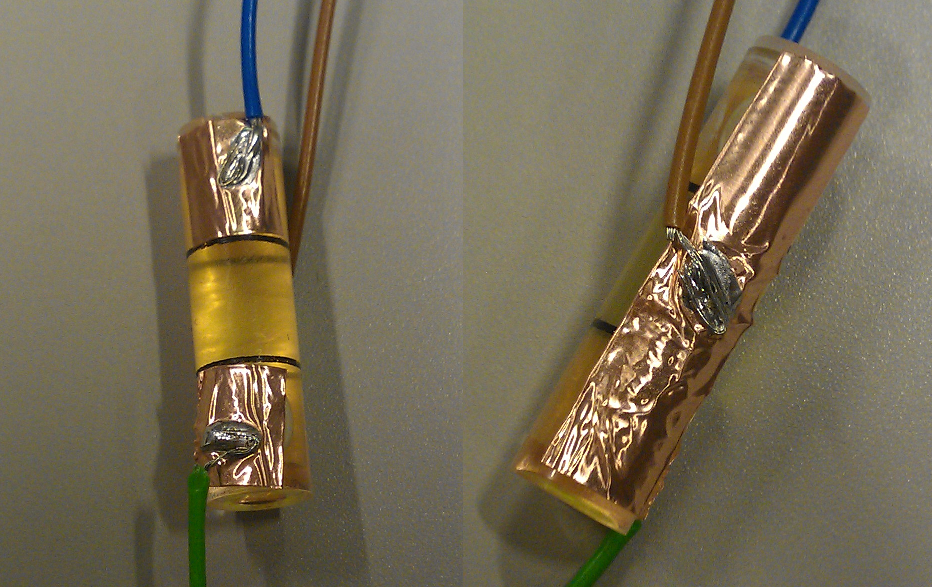
\includegraphics[width=0.5\textwidth]{billeder/libellesensor1}
\caption{henning}
\label{fig:libelle}
\end{figure}
Vi kom frem til at den har en capacitet på omkring $1*10^{-15}[F]$. Det gør det praktisk umuligt at anvende da vores filter så har en alt for stor cutoff frekvens liggende over 3.0 MHz. Den høje frekvens giver en stor selvinduktion i vores ledning. Samtidig kan vi ikke lave sinus med denne frekvens med PSoC'en. Dette gjorde at vi måtte finde en anden løsning.\\
Næste prototype bestod af et potmeter og et pendul. Dog havde potmeteret en for stor friktionsmodstand, der gjorde det upræcist i forhold til vores krav.\\
Vi har gennem et tredje semestersfag fundet ud af at PSoC'en indeholder et accelerometer. Vi valgte så at lave en prototype med det. Dette viste sig at være en god løsning.